\begin{comment}
\subsection{Análise Formal}
\label{AnlForm}

O problema apresentado retrata-se num tradicional problema resolvido por um método de pesquisa exaustiva de verificar, de todas as combinações de $n$ vértices do grafo, quais satisfazem a condição, o que se traduz logo à partida numa complexidade de $\mathcal{O}(2^n)$. No contexto deste problema, cada vértice tem apenas duas possibilidades, estar presente no conjunto dominante ou não.

Posto isto é necessário analisar todas as combinações de tamanho $k$, de 1 até $n$. A cada combinação $i$ é preciso analisar se os vértices são vizinhos. Isto traduz-se em 2 somatórios, um $j$ começando no primeiro vértice e indo até ao penúltimo vértice, $k-1$, e o outro somatório começando em $j+1$ indo até ao elemento, $n$.

Assim, no total, temos então 4 somatórios, os dois mais exteriores para gerar as combinações de tamanho $k$, de 1 até $n$, e os dois mais interiores, para verificar se os vértices são vizinhos ou não. Estes somatórios são representados como de seguida:

\[
\sum\limits_{k=1}^{n}\sum\limits_{i=1}^{n \choose k}\sum\limits_{j=1}^{k-1}\sum\limits_{g=j+1}^{k} 1 = 2^{n-3}(n-1)n
\]

Podemos simplificar o resultado para uma mais fácil visualização,
\[
2^{n-3}(n-1)n = \frac{2^{n}}{2^3}(n^2 - n) = \frac{1}{2^3}(n^2 \times 2^{n} - n\times 2^{n})
\]


O que se traduz então numa complexidade computacional de $n^{2}\times 2^{n}$, $\mathcal{O}(n^{2}\times 2^{n})$.


\begin{figure}[h!]
    \centering
    \subfloat[\centering]{{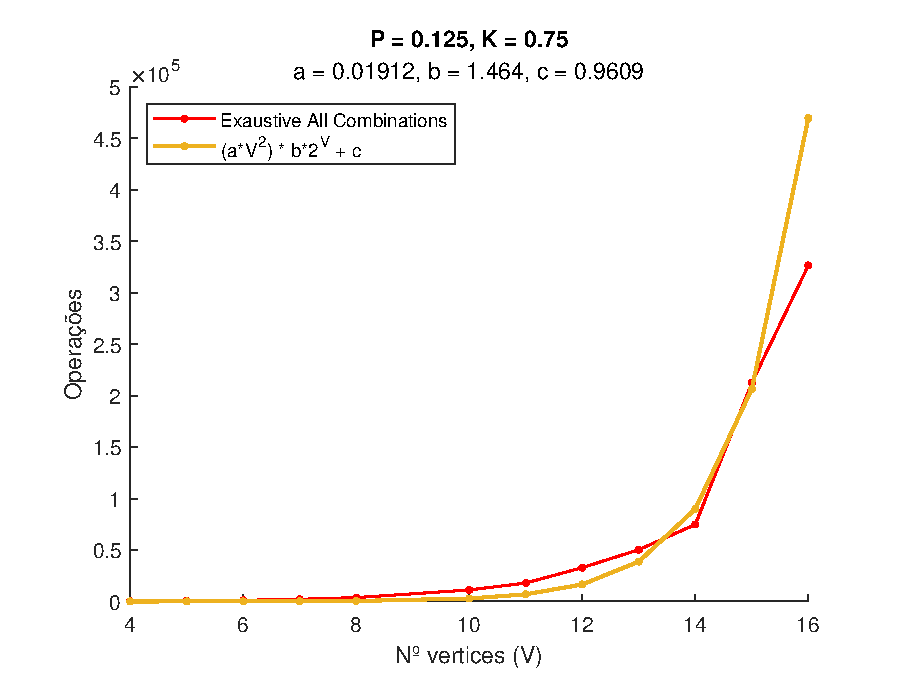
\includegraphics[scale = 0.5]{Figs/fit.eps} }}%
    \qquad
    \subfloat[\centering]{{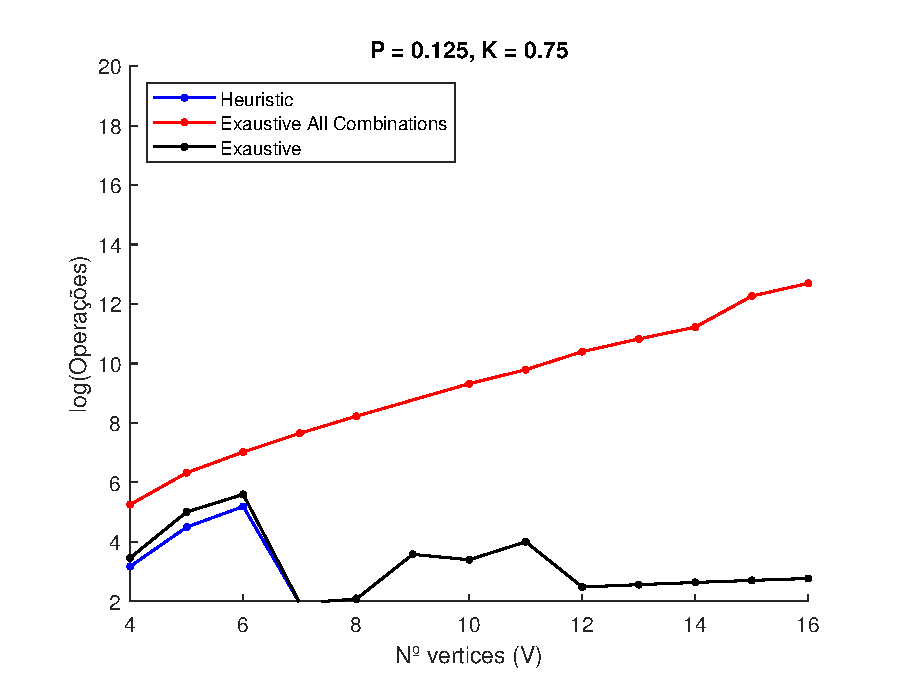
\includegraphics[scale = 0.5]{Figs/fit2.eps} }}%
    \caption{(a) Fit ($R^2 = 0.96$) ao número de comparações realizadas pelo algoritmo exaustivo que verifica todas as combinações e (b) Logaritmo do número de operações, em função do número de vértices, realizadas pelos 3 algoritmos - $P = 0.125, K = 0.75$}%
    \label{Allcomb}%
\end{figure}

Foi desenvolvido um código de pesquisa exaustiva que analisa todas as  combinações, mesmo aquelas que se sabe que não podem ser solução, pois têm um comprimento diferente de $K\times V$, de forma a poder confirmar que este problema segue uma distribuição $n^{2}\times 2^{n}$ que, como se pode ver na Fig.\ref{Allcomb} (a), assim acontece. Já na Fig.\ref{Allcomb} (b) podemos comparar a diferença com que o logaritmo do número de operações cresce em função de $V$, entre os diferentes algoritmos desenvolvidos. É possível verificar que ao apenas analisar os conjuntos que representam uma solução possível (Exaustiva) a complexidade computacional diminui, o que nos permite resolver este problema para grafos de dimensões maiores.
\end{comment}